\section{Aritmatika Pointer dan Skalasi}

Aritmatika pointer dalam bahasa tingkat tinggi seperti C diterjemahkan ke dalam kalkulasi alamat otomatis oleh kompilator yang menyesuaikan ukuran tipe data.

\subsection{Hubungan Pointer dan Skala}
Saat kita melakukan \code{p + i} di mana \code{p} adalah pointer ke tipe data $T$, alamat fisik yang dihitung adalah:
\[ \text{Alamat Baru} = \text{Alamat Lama} + (i \times \text{sizeof}(T)) \]
Kompilator secara otomatis menyisipkan faktor skala (\textit{scale factor}) ini ke dalam instruksi mesin.

\subsection{Kaitan dengan Addressing Mode}
Pada arsitektur mesin, operasi pointer seringkali dipetakan langsung ke mode pengalamatan terindex.
\begin{itemize}
    \item \textbf{High-Level}: \code{int val = *(ptr + i);}
    \item \textbf{Machine-Level (x86)}: \code{MOV EAX, [EBX + ECX*4]}
\end{itemize}
Di sini, \code{EBX} adalah \code{ptr}, \code{ECX} adalah \code{i}, dan faktor skala 4 adalah \code{sizeof(int)}.

\subsection{Pointer vs Array}
Bagi kompilator, array dan pointer seringkali diperlakukan dengan logika pengalamatan yang identik. Nama array bertindak sebagai alamat dasar (\textit{base address}) konstanta, sedangkan pointer adalah alamat dasar variabel.
\begin{itemize}
    \item \code{A[i]} $\equiv$ \code{*(A + i)}
    \item Kompilator menggunakan informasi tipe data untuk menentukan apakah ia harus melompat 1 byte (\texttt{char}), 4 byte (\texttt{int}), atau 8 byte (\texttt{double}) untuk setiap penambahan indeks.
\end{itemize}

\begin{figure}[!htbp]
    \centering
    \adjustbox{max width=0.8\textwidth,center}{%
    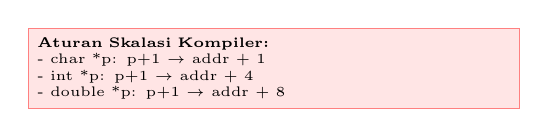
\begin{tikzpicture}[
        node/.style={rectangle, draw=red!50, fill=red!10, text width=6cm, font=\tiny}
    ]
    \node[node] (scal) {
        \textbf{Aturan Skalasi Kompiler:}\\
        - \code{char *p}: \code{p+1} $\rightarrow$ \code{addr + 1}\\
        - \code{int *p}: \code{p+1} $\rightarrow$ \code{addr + 4}\\
        - \code{double *p}: \code{p+1} $\rightarrow$ \code{addr + 8}
    };
    \end{tikzpicture}%
    }
    \caption{Skalasi Otomatis dalam Aritmatika Pointer}
\end{figure}
